\documentclass[a4paper, 10pt, conference]{ieeeconf}    

\usepackage{caption, graphicx, amsmath, tabularx, indentfirst, lastpage, dsfont}    
\usepackage{fancyhdr}
\pagestyle{fancy}
\fancyhf{}
\renewcommand{\headrulewidth}{0.4pt}
\renewcommand{\footrulewidth}{0.4pt}
\cfoot{\thepage\ of 5}                                   
                                                       
\IEEEoverridecommandlockouts
\overrideIEEEmargins
\usepackage{float}
\floatstyle{ruled}
\restylefloat{figure}  
\restylefloat{table}    
\title{\Large \bf Understanding the Effects of Drugs on Criminal Behaviors and Emotional Stress, using Coarsened Exact Matching, Doubly Robust Regression and Bayesian Additive Regression Trees, an Observational Study}
\author{Darshan Patel}

\begin{document}
\maketitle
\thispagestyle{fancy}
\begin{abstract}

To understand the association between smoking cigarette and marijuana and criminal behaviors and emotional stress indicators. The criminal acts studied here are theft, arson and burglary. Signs of emotional stress that were studied include nervousness, hopelessness and worthlessness. Methods explored in this investigation are coarsened exact matching to match observations for logistic modeling, as well as doubly robust regression and BART to find average treatment effects. It was found that smoking cigarette and criminal behavior were related, as well as smoking marijuana and emotional stress indicators. 
\end{abstract}

\section{INTRODUCTION}

The use of drugs is a public health problem all over the world. This is of interest for two reasons. One is, the rise of criminal behaviors when indulging in drugs. whereas the other is the indication of mental stress. 

Common crimes that get committed include motor vehicle theft, burglary, arson, DUI, sexual offense, fraud and other violent offenses. There are several factors that can indicate why people undergo these criminal behaviors. From having relationship issues, to financial problems, or feeling of insecurity, people over time have committed crimes to get what they want. An underlying reasoning can also be whether they were in the influence of drugs. For instance, DUI is abbreviation for driving under influence; one can only get committed for this when definitely under the influence of alcohol and drugs. But a more subtle relationship can be dug for other crimes. 

Apart from committing crimes, people often take drugs when they were not feeling good mentally. When one is feeling down due to family problems, school pressure or financial issues, they look to drugs to take away the stress for a temporary amount of time. For instance, in high school, many students enjoy smoking marijuana during school hours to relieve themselves. Signs of mental stress include anxiety, isolation, moodiness, unhappiness and more. 

In this paper, several criminal offenses and mental stress indicators will be studied. The crimes that are looked at theft, arson and burglary. Emotional stress indicators that are looked at are feelings of nervousness, hopelessness and worthlessness. An observational study will be done comparing the use of cigarette and marijuana in 2017 to determine whether taking drugs is indicative of someone having committed a crime or having an indication of emotional stress. Methods explored are coarsened exact matching, doubly robust regression and Bayesian additive regression trees. 


\section{Data}

The data provided for this study will come from the National Survey of Drug Use and Health, done in 2017. In the study, the purpose of the survey was to measure the prevalence of drugs in the United State and find relevant information about users and non-users. The target subject for the survey is the civilian, non-institutionalized population of the United States, who are older than 12 years at the time of the survey. The survey was done using CAI methods as well as holding minimum sample sizes per state. Demographic subgroup estimates were also made due to the large sample sizes. In the year of the study, $56, 276$ subjects were interviewed. Furthermore, drugs focused on include tobacco, marijuana, crack, cocaine, hallucinogens, heroin, inhalants, methamphetamine, pain relievers, tranquilizers, stimulants and sedatives. Various information about each drug were collected, such as whether the subject has ever taken them and if so, what age did they first try it, time since they last did it, the frequency of use in the past week, month and year, and more. For specialization, information about different strands of drugs were also noted if the drug label was big. For instance, hallucinogens was broken down into LSD, PCP, mescaline and more. Apart from drug usages, information on peoples' social environment, youth experiences, mental health, depression, consumption of alcohol, substance dependence and abuse, criminal acts, and drug treatment was also surveyed. A total of more than $2,500$ variables of information was collected or derived from survey participants. 

To aid this study, and optimize computational performance, a handful of variables were extracted. The drugs that was focused on are cigarette, a form of tobacco, and marijuana. Only if a subject has or has not taken the drug in their lifetime was of concern; meaning, there was surety in the drug usage. In Table I, the the number of smokers and non-smokers for both cigarette and marijuana is shown. 

% latex table generated in R 3.4.3 by xtable 1.8-3 package
% Wed Apr 17 15:42:07 2019
\begin{table}[ht]
\centering
\begin{tabular}{rlrr}
  \hline
 & Yes/No & Cigarette & Marijuana \\ 
  \hline
1 & No & 28971 & 32031 \\ 
  2 & Yes & 27305 & 24214 \\ 
   \hline
\end{tabular}
\caption{Usage of Cigarette and Marijuana}
\end{table}


\parindent 10pt From here on outwards, the control group is the group of subjects that don't smoke the drug whereas the treatment group is the group of subjects that do indulge in the drug. It can be seen that there are slightly more non-cigarette smokers than actual cigarette smokers. The difference for marijuana usage is more profound; there are nearly one-third more non-marijuana smokers than actual marijuana smokers. To study criminal offenses, a combination of three variables will be focused on: whether a subject has been arrested and booked for theft in the past $12$ months, and likewise for arson and burglary. To reduce the number of models to make, an indication variable will be created that represents all three of these crimes. If an individual has committed one or more of these three crimes, their value will be $1$, otherwise $0$, indicating no criminal behavior. The same technique will be utilized for the emotional stress indicators. The ones that are looked at in this study are: nervousness, hopelessness and worthlessness. If an individual has felt one (or more) of these feelings heavily during a particular month in 2017, their value will be $1$, otherwise $0$. 

A few covariates, or demographic information will be needed for this study to understand the effect of drugs. The demographic information that was used in this study are gender, age, race and employment status. A percentage distribution of these demographics features for cigarette users is shown in Fig. 1. 
\begin{figure} 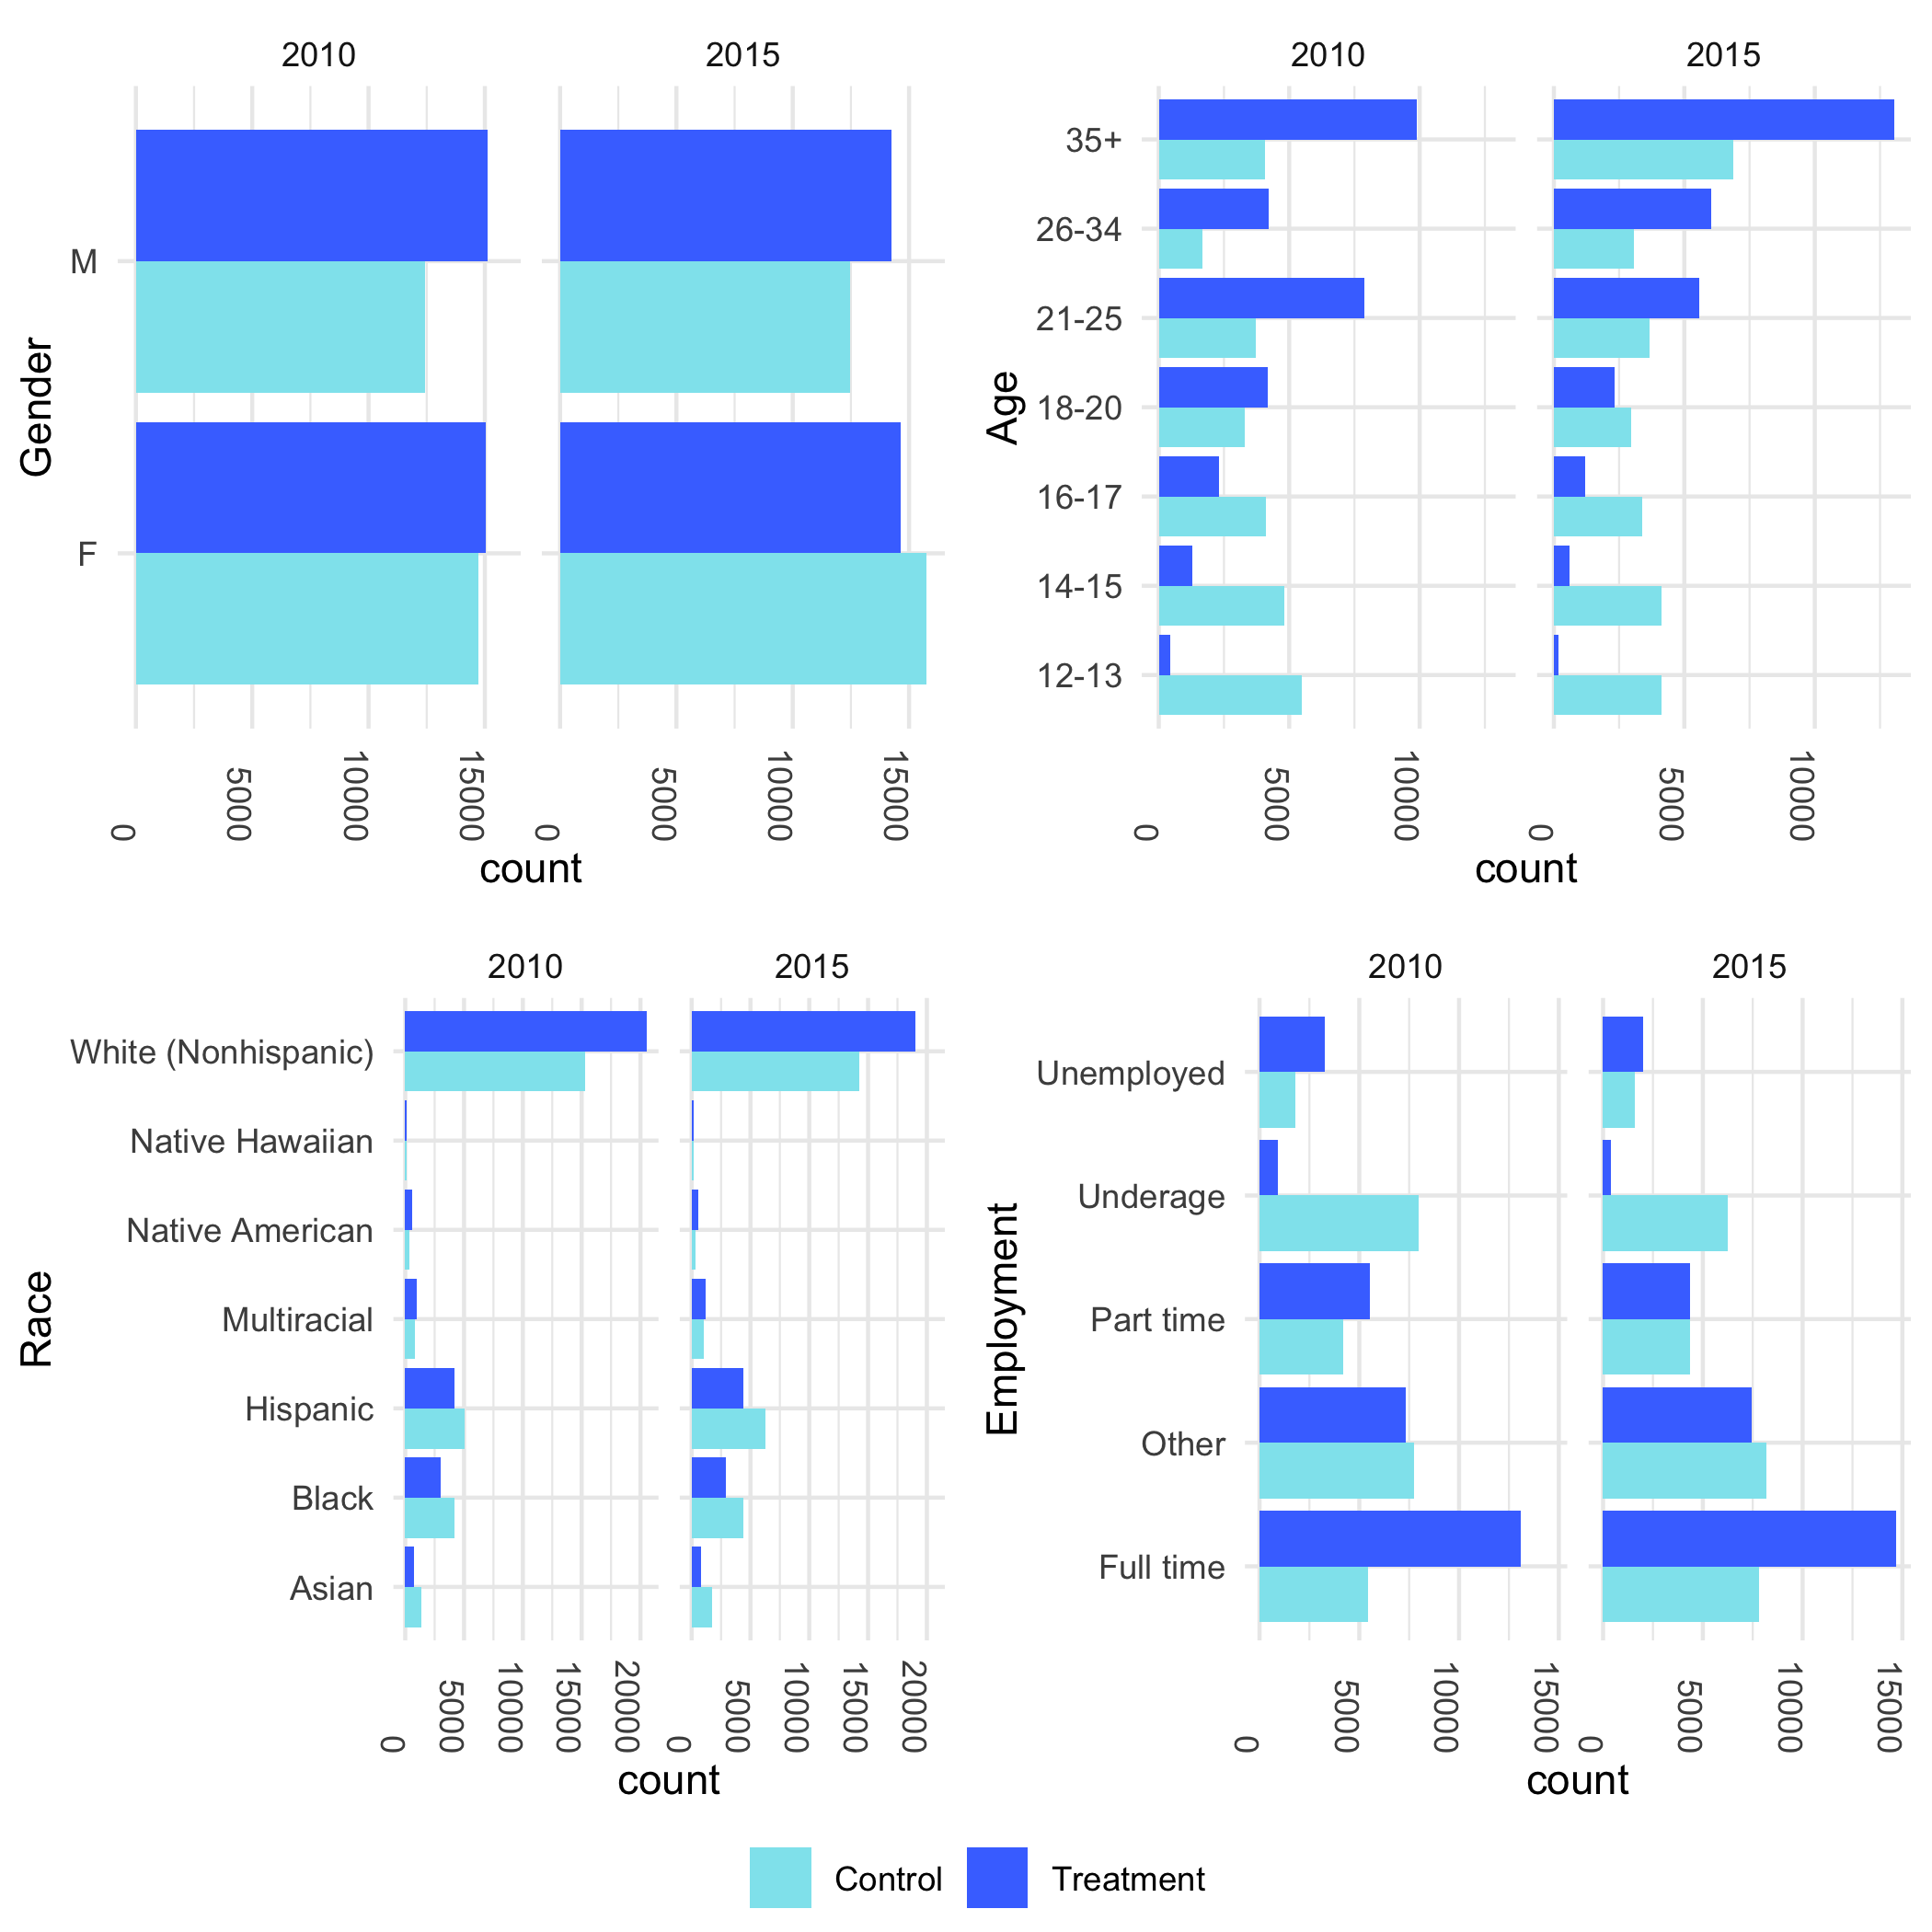
\includegraphics[scale = 0.11]{CigaretteDemographics} \captionof{figure}{Demographic Breakdown of Cigarette \\ } \end{figure} 
\parindent 10pt In this plot, the control group is the subjects who did not smoke cigarette, while the treatment group is the subjects who did. There are several takeaways from this analysis. 
First, the percentage of men and women who smoked cigarette is nearly the same. This contrasts with the fact that there are less male non-smokers than female non-smokers. Looking at the age percentage distribution, the $35+$ age group holds most of the population. As age increases, there is a growth in the percentage of cigarette users in the study while non-smokers decreases slighly until a jump at $35+$ years old. There is a huge imbalance in racial demographics in this study, where non-hispanic whites make up more than $50\%$ of the study, leaning more heavily on the cigarette user side. Lastly, it is noted that that this study there are more cigarette users who are full-time workers than those who do not; an entire $25+\%$ of the study is made up of full-time employees who smoke cigarette. This contrasts with the other employment status where percentage of non-smokers exceeds percentage of smokers. What is interesting is that unemployed people make up the lowest proportion of the study and yet have equal percentage on both sides. 

A similar analysis can be done for marijuana smokers. 
\begin{figure} 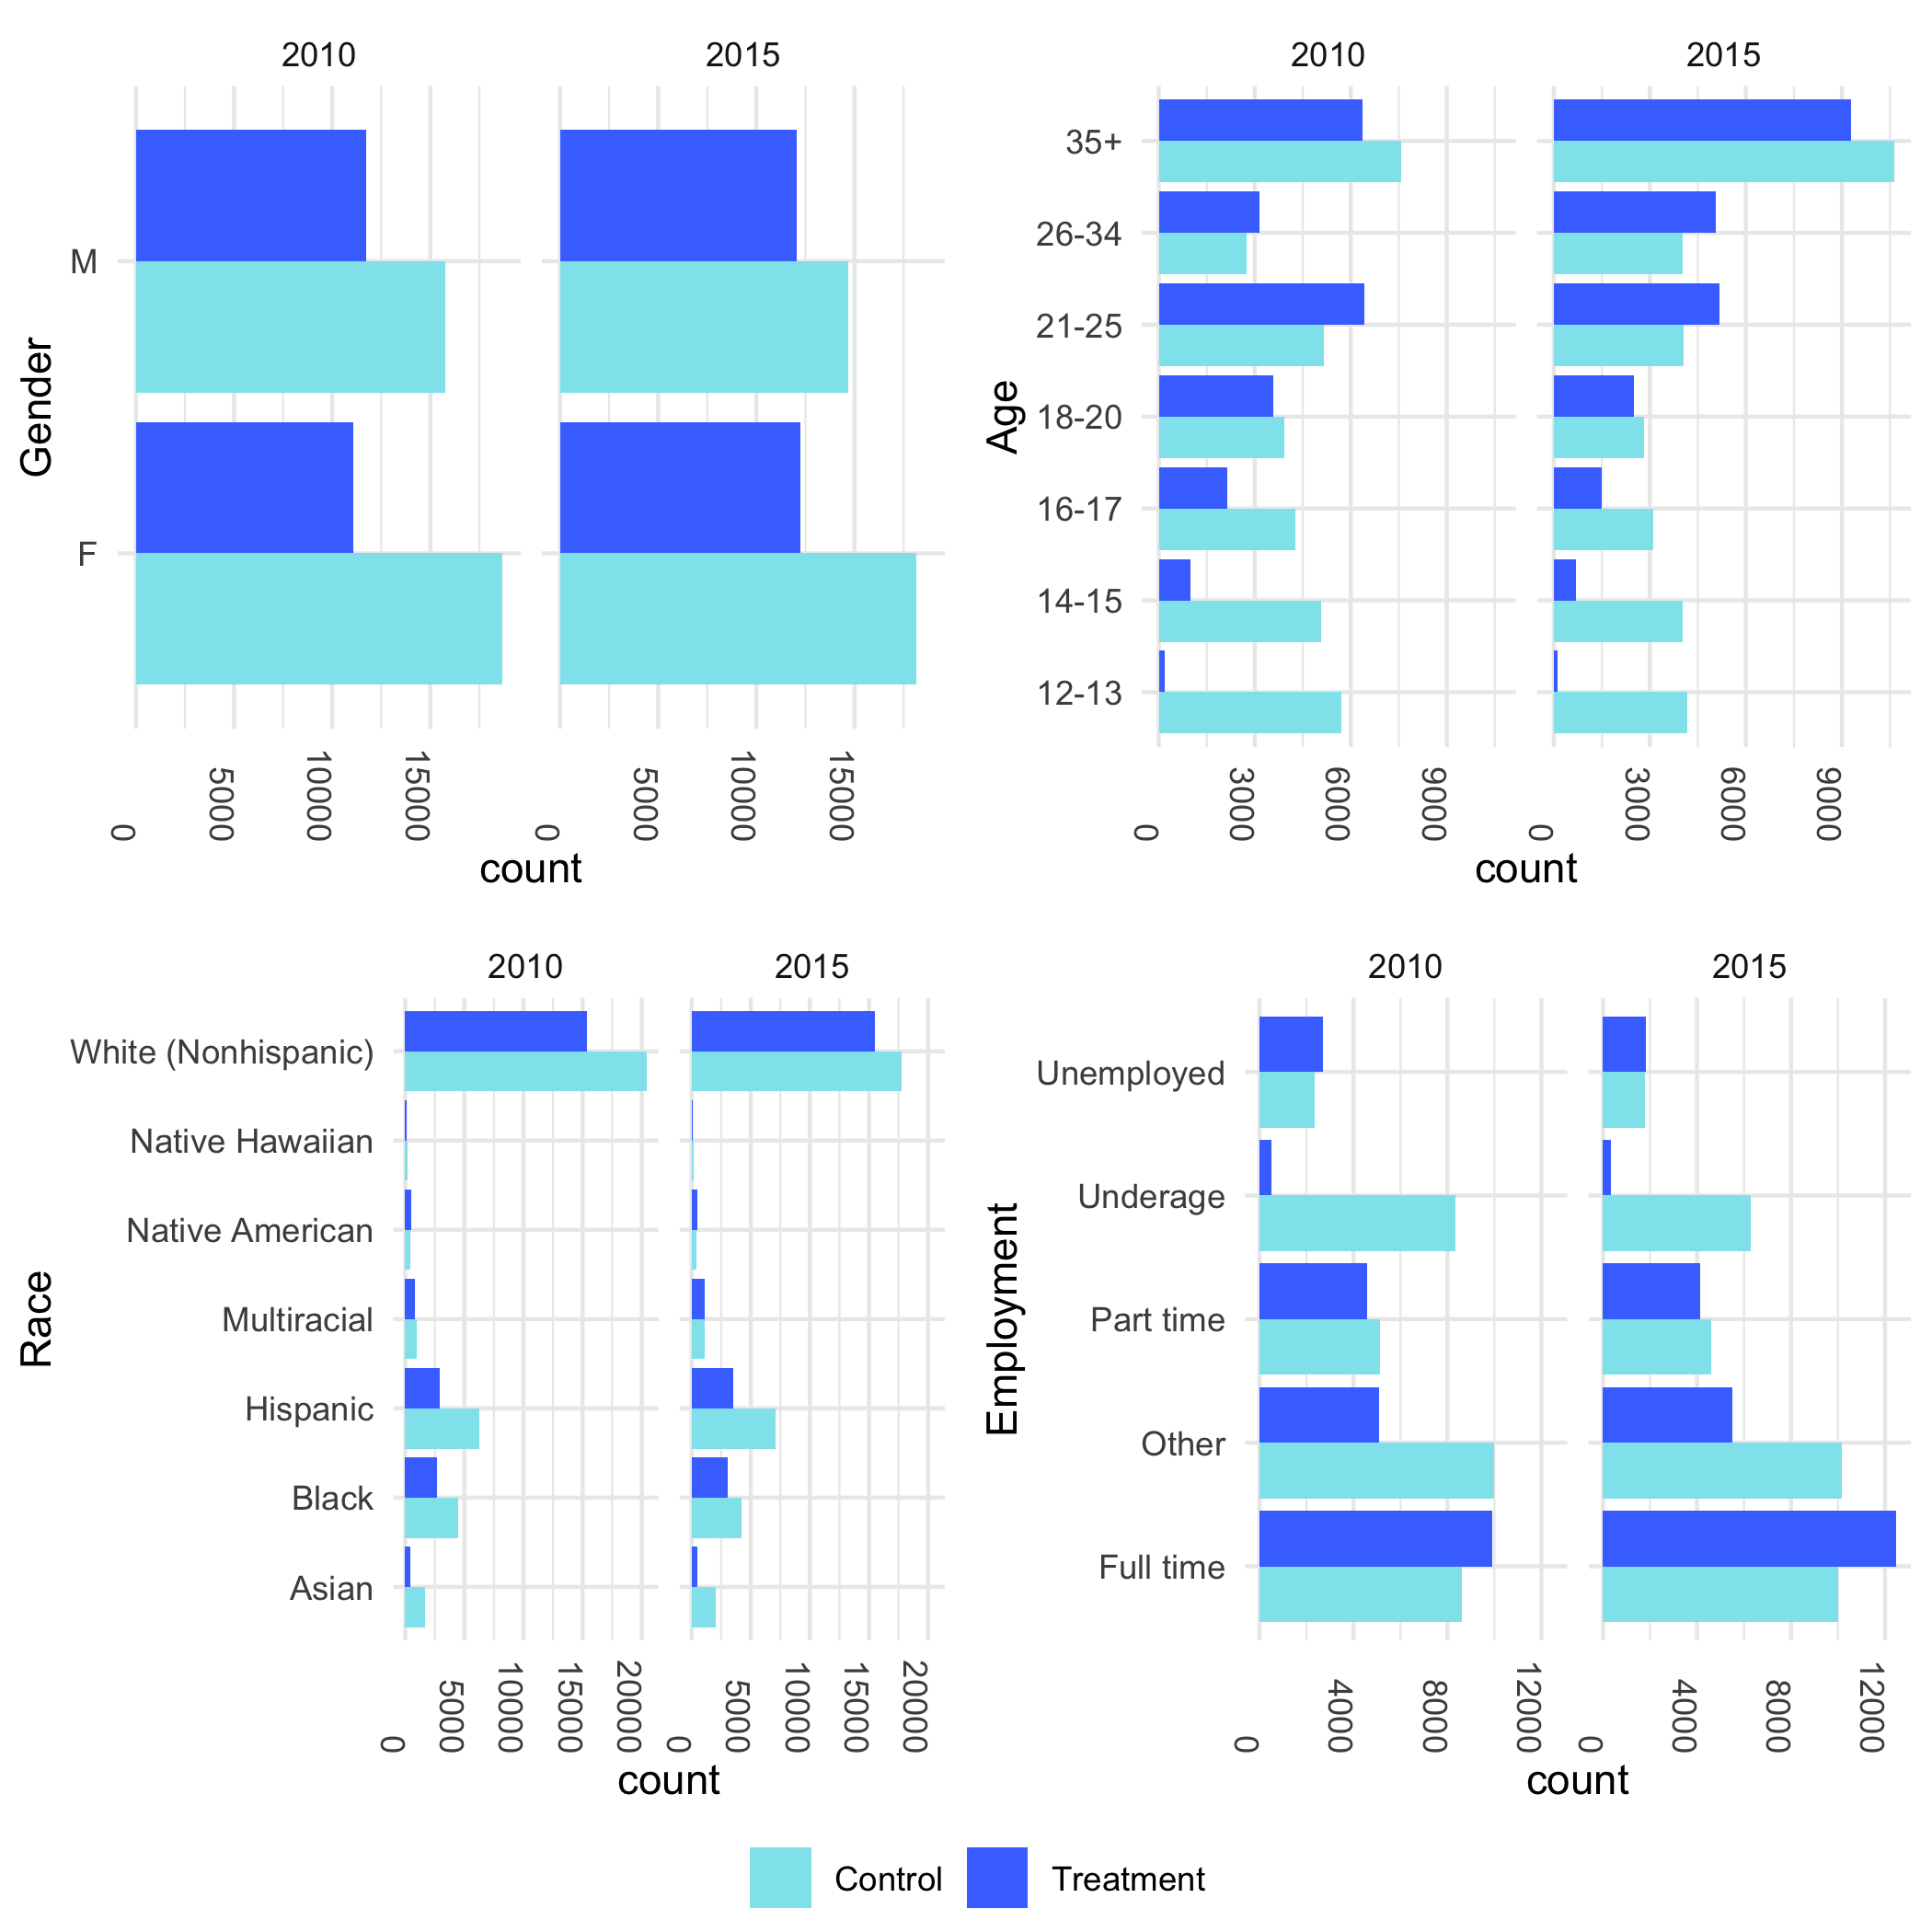
\includegraphics[scale = 0.11]{MarijuanaDemographics} \captionof{figure}{Demographic Breakdown of Marijuana \\ } \end{figure} 
\parindent 10pt A breakdown of the demographics features for marijuana use is shown in Fig. 2. The control group refers to people who have not smoked marijuana whereas the treatment group refers to people who have smoked marijuana. It is seen here that there are equally $\approx 20\%$ of marijuana smokers who are male and $\approx 20\%$ that are female. The other $60\%$ is distributed unevenly non-smokers of both genders. As for age, almost $40\%$ of the participants are $35$ years or older. In addition, the percentage of marijuana smokers and non-marijuana smokers is almost identical in that age group. In fact, the percentage for $26$ to $34$ between both groups is nearly equal as well. A total of three age groups appears to have similar distribution in groups. Looking at race, the white demographic continues to be the majority group, making up half of the population. However in this case, the non-marijuana smoker group is slightly larger than the marijuana smoker group. The number of hispanic and black people make up twice as much in the population of non-smokers than in the population of smokers. Late but not the least, there is nearly an equal distribution between the full time smokers and full time non-smokers, and likewise for part time workers. 

\section{Methods} 
\parindent 10pt After setting up the indicator variables and analyzing the data, modeling can proceed. For the first phase of this study, coarsened exact matching will be performed to match observations of differing treatments. The CEM algorithm is as follows: first each covariate is coarsened as much as possible. Then each observation is sorted into stratas defined by the coarsening. Finally, observations in any stratum that do not include both treatment/non-treatment groups are pruned (or excluded). This is a principle stratification process. Using the stratified observations, the average treatment effect is computed using a logistic model approach. Coefficients from the model are interpreted in terms of odds ratios. These interpretations are compared with a model where extrapolation is performed (meaning all data is used to estimate the model). For the second phase of this study, doubly robust regression models are created on bootstrapped samples to create estimates of the average treatment effect. After running the bootstrap over $1000$ iterations, a confidence interval is created on the ATE estimates. For the third and final phase of this study, Bayesian additive regression trees are created to calculate the average treatment effects. A total of $200$ trees are created over $1100$ iterations of the Markov chain Monte Carlo process for each model. Using the mean and standard deviation of the ATE estimates, a confidence interval is created. This confidence interval is compared with the one created from the doubly robust regression models. Hypothesis testing is also done to determine whether the average treatment effect estimates are statistically significant.

\section{Results}
\subsection{Coarsened Exact Matching}
In Table II, the percentage of matched and unmatched subjects are shown. 
% latex table generated in R 3.4.3 by xtable 1.8-3 package
% Mon Apr 29 22:27:56 2019
\begin{table}[ht]
\centering
\begin{tabular}{rrrrr}
  \hline 
 & \small $\%$ NS M & \small $\%$ NS NM & \small $\%$ S M & \small $\%$ S NM \\ 
  \hline
Cig / C & 0.872 & 0.127 & 0.730 & 0.269 \\ 
  Mar / C & 0.929 & 0.075 & 0.738 & 0.261 \\ 
  Cig / S & 0.998 & 0.001 & 0.992 & 0.007 \\ 
  Mar / S & 0.996 & 0.003 & 0.992 & 0.007 \\ 
   \hline
\end{tabular}
\caption{Percentage of nonsmokers and smokers matched and not matched after coarsened exact matching.}
\end{table}

When matching is performed, a person who is not a smoker is matched with a person who does smoke. By coarsening on the covariates, most of the data does get properly matched. When building models to detect stress levels, over $99\%$ of the subjects are matched, regardless of whether smoke or not smoke cigarette or marijuana. This contrasts with the criminal behavior models where $93\%$ of the non-marijuana smokers are matched and the other situations have lower matching percentages. In fact, only $73\%$ of cigarette smokers are matched when looking at criminal behavior. \\~\\
In Table III, the coefficients calculated from running a logistic regression model to predict criminal behavior / stress level is shown. 
% latex table generated in R 3.4.3 by xtable 1.8-3 package
% Mon Apr 29 22:47:29 2019
\begin{table}[ht]
\centering
\begin{tabular}{rrrrr}
  \hline
 & Coef (m) & Int. & Coef (all) & Int. \\ 
  \hline
Cig / C & 0.294 & 34.264 & 0.223 & 25.040 \\ 
 Mar / C & 0.108 & 11.487 & 0.084 & 8.812 \\ 
 Cig / S & 0.224 & 25.121 & 0.222 & 24.915 \\ 
 Mar / S & 0.391 & 47.981 & 0.389 & 47.588 \\ 
   \hline
\end{tabular}
\caption{Logistic regression coefficient and interpretation using matched data and all data.}
\end{table}

The interpretation of the coefficient of estimate was derived as follows. Suppose a logistic model is created as $$ \log \left( \frac{\pi}{1-\pi} \right) = \beta_0 + \beta_1x_1 + \dots + \beta_px_p $$ where $\pi = \mathds{P}(y = 1)$ and $\log \left( \frac{\pi}{1-\pi} \right)$ is the log odds. Then $\hat{\beta}_j$, where $j > 0$, is the change in log-odds for every one unit increase in $x_j$ holding all other $x$'s fixed. A meaningful interpretation is formed by $$ (e^{\hat{\beta}_j} - 1) \times 100\%$$ which is the change in odds $\frac{\pi}{1-\pi}$ for every unit increase in $x_j$ holding all other $x$'s fixed. This formula was used to find the interpretations of the coefficients in the logistic models above. \\~\\
A number of observations are made here. The largest interpretation value is $47.981$, marijuana smokers and stress level. If a person is to smoke marijuana, then the odds of that person showing signs of stress increases by $47.981\%$, holding all covariates constant. That is nearly $50\%$! When comparing this value to the one found from creating a model on the entire dataset, the interpretation only differs by $0.4\%$. Matching did not help to find new insights here. This contrasts in the model that predicts criminal activity amongst cigarette users. When considering matched subjects, if a person is to smoke cigarette, then the odds of that person committing theft/arson/burglary rises by $34.264\%$, holding covariates constant. When running this same model on all the subjects, the percent rise is only $25.040\%$. Matching helps to see that smoking can actually increase likelihood of committing a crime. A similar analysis can be done for the other two models. Note that the differences between the interpretations for matched and all observations does not differ by a huge amount.

\subsection{Doubly Robust Regression}
The average treatment effect is a measure used to compare treatments in randomized experiments. It measures the difference in mean outcomes between the treatment and control groups. It is calculated by 
 $$ \tau_{\text{ATE}} = \mathrm{E}[Y(1) - Y(0)] $$ where $Y(1)$ is $1$ if a smoker committed the crime or exhibited stress and $0$ if a smoker has not. Likewise, $Y(0)$ is $1$ if a non-smoker committed the crime or exhibited stress and $0$ otherwise. After creating doubly robust regression models, the mean, standard deviation of average treatment effects for all models are shown in Table IV. A $95\%$ confidence interval of these estimates is also given. 
% latex table generated in R 3.4.3 by xtable 1.8-3 package
% Tue Apr 30 10:35:36 2019
\begin{table}[ht]
\centering
\begin{tabular}{rrrl}
  \hline
 & $\bar{x}_{\text{ATE}}$ & $s_{\text{ATE}}$ & Conf. Int. \\ 
  \hline
Cig / C & 0.02051 & 0.00238 & (0.01584, 0.02519) \\ 
  Mar / C & 0.03030 & 0.00223 & (0.02593, 0.03466) \\ 
  Cig / S & 0.03349 & 0.00199 & (0.0296, 0.03739) \\ 
  Mar / S & 0.04867 & 0.00202 & (0.04471, 0.05263) \\ 
   \hline
\end{tabular}
\caption{Doubly robust regression models mean ATE, standard deviation ATE and $95\%$ confidence intervals.}
\end{table}


To interpret these values, note that a positive value indicates that taking the drug increases the chances of committing a crime or exhibiting a stress indicator. Now, all four models have positive ATE estimates. The largest ATE estimate is for marijuana smokers having stress. There is a $95\%$ chance that the confidence interval ($0.044, 0.052$) contains the true average treatment effect. The smallest ATE estimate is for cigarette smokers exhibiting criminal behaviors. There is a $95\%$ chance that the confidence interval ($0.015, 0.025$) contains the train average treatment effect. Similar analysis can be done for the other two models. Note also that the standard deviation of all the estimates are $\approx 0.002$. Furthermore, the error of the criminal behavior models were slightly larger than the ones for the stress indicator models. 

\subsection{BART}
In this phase of the study, BART models were created and a confidence interval was calculated for the average treatment effect estimates. This is shown in Table V. 
% latex table generated in R 3.4.3 by xtable 1.8-3 package
% Tue Apr 30 10:35:25 2019
\begin{table}[ht]
\centering
\begin{tabular}{rrrl}
  \hline
 & $\bar{x}_{\text{ATE}}$ & $s_{\text{ATE}}$ & Conf. Int. \\ 
  \hline
Cig / C & 0.07418 & 0.00012 & (0.07395, 0.07441) \\ 
  Mar / C & 0.14108 & 0.00012 & (0.14085, 0.1413) \\ 
  Cig / S & 0.12657 & 0.00003 & (0.12652, 0.12663) \\ 
  Mar / S & 0.21515 & 0.00003 & (0.2151, 0.2152) \\ 
   \hline
\end{tabular}
\caption{BART models mean ATE, standard deviation ATE and $95\%$ confidence interval.}
\end{table}


The largest ATE estimate goes to the marijuana smokers exhibiting stress. The smallest ATE estimate goes to the cigarette smokers exhibiting criminal activity. This was similarly seen in the comparison of the robust regression model ATE estimates. Note that now the mean estimates are larger and the standard deviations are even smaller, less than $0.0002$.
\\~\\
A plot of the confidence intervals is shown below in Fig. 3.
\begin{figure} 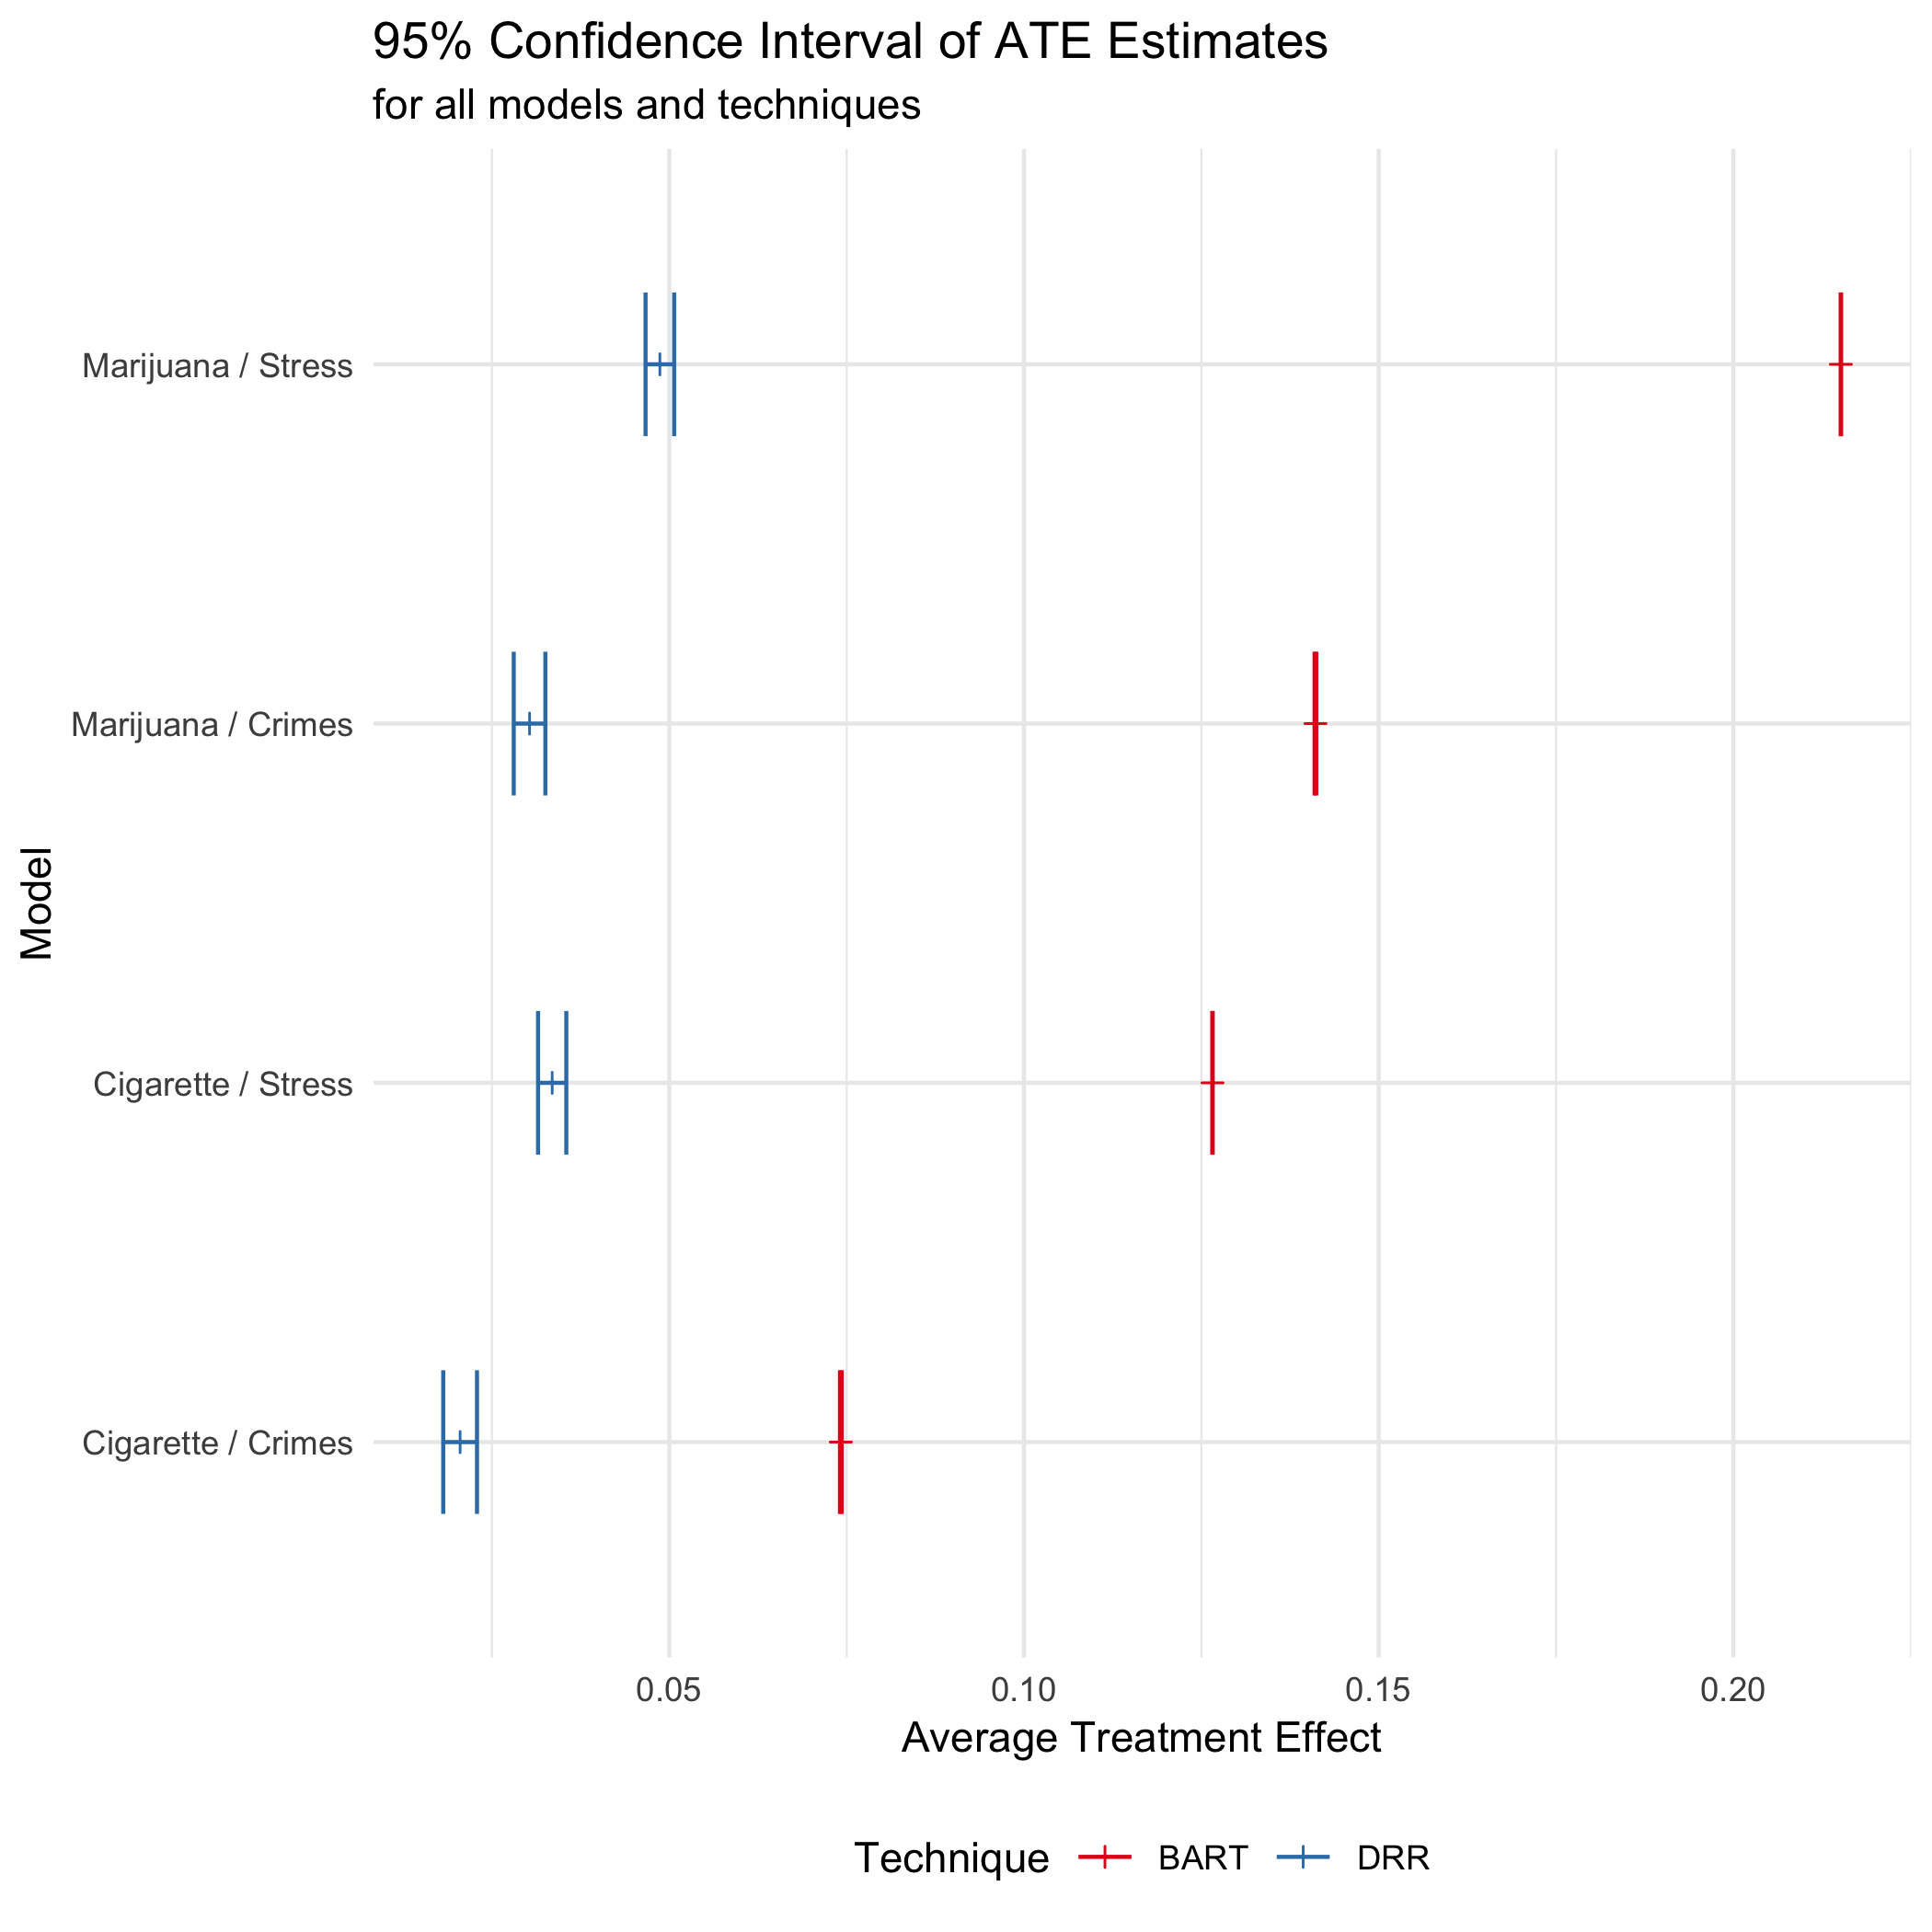
\includegraphics[scale = 0.1]{ATEplot}\captionof{figure}{Plot of $95\%$ confidence intervals.} \end{figure}
It is clear that the BART models estimated the average treatment effect with better accuracy than the doubly robust regression models, due to the minuscule standard error. Furthermore, it calculated a higher average treatment effect for all of the models. The robust regression models were created by manually bootstrapping samples of size $200$ and creating estimates whereas the BART models bootstrapped the samples based on its own algorithm. 

\subsection{Hypothesis Testing}
To evaluate whether these average treatment effects were statistically significant, a Neyman hypothesis test was conducted. Under the Neyman's framework, let the null hypothesis state that the average treatment effect is zero, or 
$$ H_0: \mathrm{E}[Y(1) - Y(0)] = 0 $$ Note that this hypothesis is different from Fisher's sharp null hypothesis which assumes each unit has zero treatment effect. Now, the alternative hypothesis is that the average treatment effect is not zero, or $$ H_A: \mathrm{E}[Y(1) - Y(0)] \neq 0 $$ To test these hypotheses, a $t$ statistic is calculated as follows
$$ t = \frac{\tau_{\text{ATE}}}{\text{Var}[\tau_{\text{ATE}}]} = \frac{\overline{Y(1)} - \overline{Y(0)}}{\sqrt{ \frac{s_1^2}{N_1} + \frac{s_0^2}{N_0}}} $$ The $p$-value is then computed for a two-sided $t$-test.  The result is shown below in Table VI.
% latex table generated in R 3.4.3 by xtable 1.8-3 package
% Sun May  5 17:52:20 2019
\begin{table}[ht]
\centering
\begin{tabular}{rllrrr}
  \hline
 Type & Model & t & df & p \\ 
  \hline
 DRR & Cig / C & 111.86 & 1396 & 0.00 \\ 
   DRR & Mar / C & 176.38 & 1396 & 0.00 \\ 
   DRR & Cig / S & 768.11 & 13532 & 0.00 \\ 
   DRR & Mar / S & 1099.70 & 13532 & 0.00 \\ 
   BART & Cig / C & 8024.30 & 1396 & 0.00 \\ 
   BART & Mar / C & 15261.09 & 1396 & 0.00 \\ 
   BART & Cig / S & 192563.10 & 13532 & 0.00 \\ 
   BART & Mar / S & 327328.40 & 13532 & 0.00 \\ 
   \hline
\end{tabular}
\caption{Neyman hypothesis testing results.}
\end{table}
 

All of the model estimates are deemed statistically significant at the $\alpha$ level of $0.05$. Therefore, the null hypothesis can be rejected and it can be ruled that the average treatment effect is not zero. The ATE estimates can be trusted more now despite being close to zero for most models.

\section{Conclusion}

In this observational study, an attempt was made to find causal relations between taking certain drugs and criminal behaviors and emotional stress indicators. This was done using three methods: coarsened exact matching, doubly robust regression and Bayesian additive regression trees. It was found that by coarsening the sample observations, most of the data become matched. By looking at matched observations, it was found that cigarette users have an increased odds of $34\%$ of committing a crime of burglary, arson or theft, when leaving all other covariates constant. The covariates used were age, gender, race and employment status. Matching however did not prove to show a huge difference in logistic regression coefficient interpretations with the other three scenarios. In the doubly robust regression phase, it was found that the mean average treatment effects were positive for all of the scenarios, the largest being for marijuana smokers exhibiting emotional stress indicators. The estimates did have huge standard errors though. This contrasts with the third phase of the study, the BART models. The mean average treatment effects found here were larger and more precise, having a lower standard deviation. In addition, the highest mean estimate was for marijuana smokers exhibiting stress. By the use of Neymen's hypothesis testing, to determine whether the mean ATE estimates were truly nonzero, it was found that all of the estimates found were statistically significant at the $\alpha$ level of $0.05$. This meant that the average treatment effects were truly not zero for any of the scenarios. 

This study could improve in several ways. More covariates could be considered, such as marital status, being in the military and sexual identity. Plenty of other demographic information is provided in the NSDUH survey given. Another consideration is the use of TMLE (targeted maximum likelihood estimation) to find the average treatment effect and average treatment effect among the treated. Computing the ATT was omitted in this study but it can be looked at. Also think about bootstrapping different sample sizes and see how that affects the ATE calculation when doing doubly robust regression modeling. In this study, some observations were made about emotional stress indicators. Consider making the variable binary using a higher threshold during data preparation and see how that changes the average treatment effect. Finally, consider looking at other drugs like ecstasy and LSD. 

\section*{Acknowledgment}

I would like to acknowledge Professor Frank Yoon, adjunct associate professor of statistics at Fordham University, for his continual effort to educate and provide feedback to students in his observational studies course, despite a low turnout.

\end{document}
